In this section we present the results of a series of experiments we have conducted using AppScale and EAGER. We mainly focus
on the extra overhead imposed by EAGER on the application deployment process, as the number of deployed APIs and dependencies
grow. We also deploy a real-world API dataset (from ProgrammableWeb.com) on AppScale and EAGER, and evaluate how a large 
volume of API metadata can influence the behavior of EAGER.

\subsection{Performance on Stock AppScale without EAGER}
Before evaluating the performance overhead of EAGER, lets take a look at how long it takes to deploy an application on stock (unmodified)
AppScale. Table~\ref{tab:sample_apps} lists a number of sample applications along with their sizes and average deployment times on AppScale.
These applications have been chosen to represent a wide range of programming languages, application sizes and business domains. The average
deployment time and standard error values were computed over 3 readings.

\begin{table*}[ht]
\begin{center}
\begin{tabular}{| l | p{6cm} | l | l | l | }
\hline
Application & Description & Size & Deployment Time (s) & Std. Error\\ \hline
guestbook-py & A simple Python web application that allows users to post comments and view them & 16K & 22.13 & 0.34 \\ \hline
guestbook-java & A Java clone of the guestbook-python app & 52M & 24.18 & 0.09 \\ \hline
appinventor & A popular open source web application that enables creating mobile apps & 198M & 111.47 & 5.75 \\ \hline
coursebuilder & A popular open source web application used to facilitate teaching online courses & 37M & 23.75 & 0.30 \\ \hline
hawkeye & A sample Java application used to test AppScale & 35M & 23.37 & 0.27 \\ \hline
simple-jaxrs-app & A sample JAXRS app that exports 2 web APIs & 34M & 23.45 & 0.34 \\ \hline
dep-jaxrs-app-v1 & A sample JAXRS app that exports a web API and has one dependency & 34M & 23.72 & 0.32 \\ \hline
dep-jaxrs-app-v2 & A sample JAXRS app that exports 2 web APIs and has one dependency & 34M & 23.95 & 0.65 \\ \hline
\end{tabular}
\end{center}
\caption{Sample AppScale Applications}
\label{tab:sample_apps}
\end{table*}

Note that the smallest deployment time recorded on AppScale is 22.13 seconds. Also there's a clear correlation between the
size of the application, its average deployment time and the standard error observed. Larger applications take longer to deploy,
and exhibits a higher standard error. This is because larger applications take longer to be transferred over the network to the 
servers in the cloud. AppScale also archives and compresses application files for deployment, which takes extra
time.

We noticed at a very early stage that the extra overhead imposed by EAGER is much smaller compared to the overall application
deployment times observed in AppScale (100's of milliseconds compared to 10's of seconds). Therefore the EAGER overhead
is too small to be observed in a plot that illustrates overall application deployment time. This caused several difficulties when it
came to analyzing the results gathered from our experiments. The strong correlation between the
application size and the variance of the deployment time was another impediment in our evaluation.

Therefore, to avoid confusion and improve the accuracy and precision of our test results, we instrumented our experiments to
only record the extra time spent on EAGER. This way we were able to better analyze the impact of number of APIs and dependencies
on EAGER overhead. Hence, in the figures that follow we only present the additional time taken by EAGER during application
deployment process.

\subsection{EAGER Overhead by Application}

Figure~\ref{fig:overhead_by_app} illustrates the extra time taken by EAGER to validate and verify the sample AppScale applications.
These results were recorded on an EAGER deployment that didn't have any policies deployed, and without any prior
metadata recorded in the API metadata manager (that is, on a clean database).

\begin{figure}
\centering
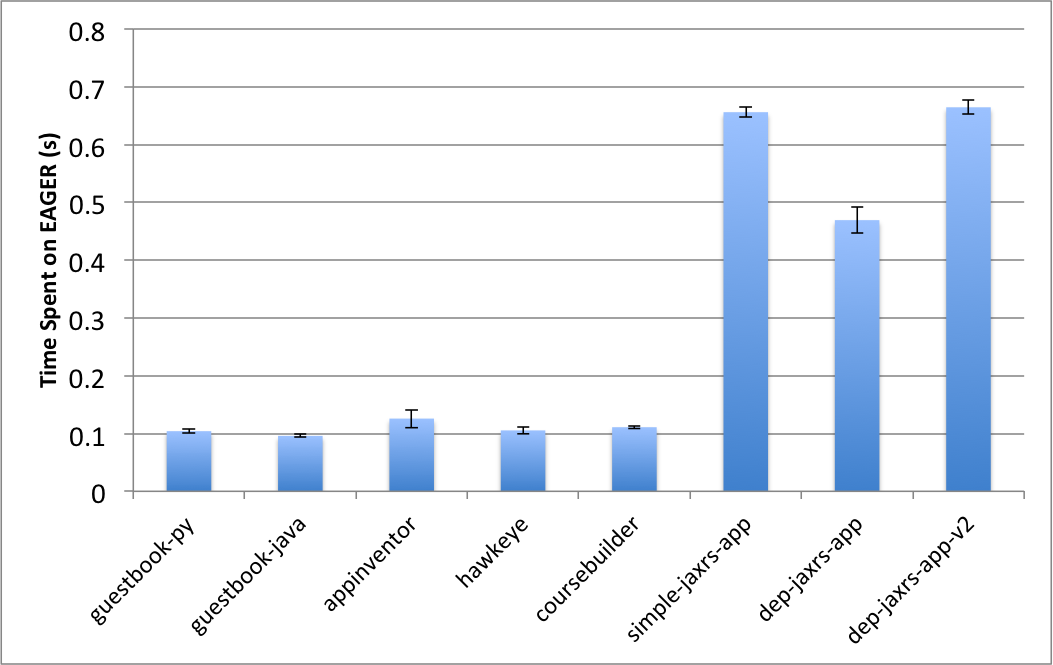
\includegraphics[scale=0.45]{overhead_by_app}
\caption{EAGER Overhead by Application}
\label{fig:overhead_by_app}
\end{figure}

Note that for the applications that do not export any web APIs, the overhead is negligibly small (around 0.1s). This is because EAGER
doesn't have to validate or record any metadata in the Metadata Manager for such applications. This implies that EAGER will not affect 
most existing AppScale apps, as long as their deployment time is concerned. For the applications that do 
export web APIs, however, EAGER has to record API metadata in the Metadata Manager, and they must be validated and published to 
the API gateway. As a result we see some extra overhead there. But even in these cases, the observed overhead is well under a second,
which is very small compared to the total application deployment time in AppScale (20+ seconds).

The overhead difference between dep-jaxrs-app-v1 and dep-jaxrs-app-v2 suggests that the EAGER overhead increases with the number
of APIs exported by an application. In the next section we will further evaluate this property.

\subsection{Impact of Number of APIs and Dependencies on EAGER Overhead}

Figure~\ref{fig:overhead_by_apis} shows that the EAGER overhead grows linearly with the number of APIs exported by an application.
This is because, in our current implementation, we iterate through the APIs in the application sequentially, and record the associated metadata in the
Metadata Manager. Then EAGER also have to publish each API to the API Gateway, so that API consumers can invoke the APIs. Since
API Gateway is a separate component, this amounts to additional web service calls, one per API. Therefore, as more and more APIs are exported 
by an application, the overhead of application deployment process via EAGER grows linearly. 

\begin{figure}
\centering
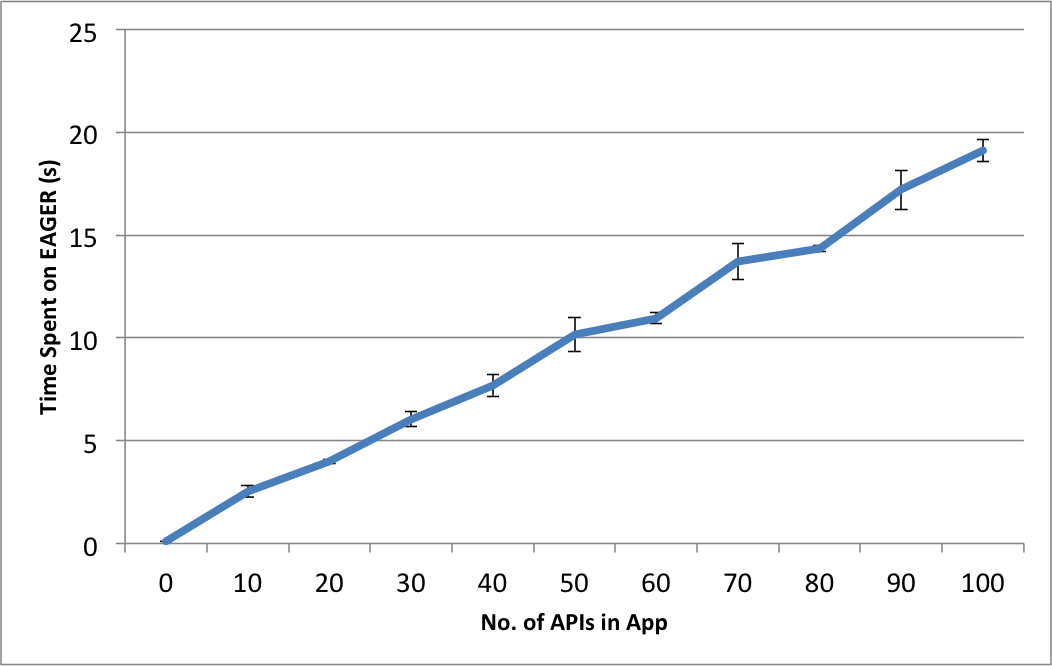
\includegraphics[scale=0.45]{overhead_by_apis}
\caption{EAGER Overhead vs. Number of APIs Exported by the Application}
\label{fig:overhead_by_apis}
\end{figure}

However, we believe that in practice this linear growth in overhead is not going to cause any serious issues for the application developers.
We expect most applications deployed in cloud to have a small to moderate number of APIs (1 to 10). According to our results, this is an 
extra overhead of 0.1-2.5 seconds, which is still very small compared to the total application deployment time of AppScale. Even in the
unlikely case of 50 APIs being exported by an application, we can only see a percentage overhead close to 30\%. It must also be noted, that
one may further improve the performance of EAGER by parallelizing the process of metadata recording and API publishing at the deployment
time. These tasks are largely independent of each other and hence there is nothing preventing them from being executed in parallel. That is,
if the developer attempts to deploy an application that exports $n$ APIs, EAGER can spawn $n$ threads where each thread will be responsible
for recording the metadata and publishing a single API.

Next, we analyze the EAGER overhead as the number of dependencies declared in an application grows. For this experiment, we first populate 
the EAGER Metadata Manager with metadata for 100 randomly generated APIs. Then we deploy an application on EAGER which exports a single
API and declares dependencies on the APIs that are already stored in the Metadata Manager. We vary the number of declared dependencies and
observe the additional overhead imposed by EAGER.

\begin{figure}
\centering
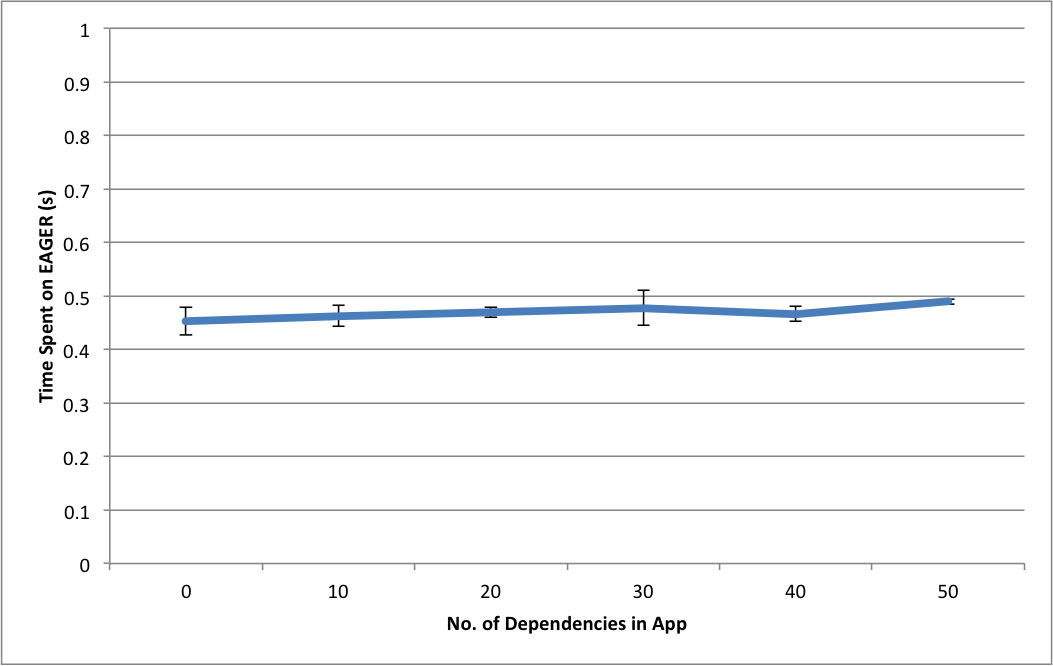
\includegraphics[scale=0.45]{overhead_by_deps}
\caption{EAGER Overhead vs. Number of Dependencies Declared in the Application}
\label{fig:overhead_by_deps}
\end{figure}

Figure~\ref{fig:overhead_by_deps} shows the results of the above experiment. According to that, the EAGER overhead is not significantly
influenced by the number of dependencies declared in an application. This is because in our current implementation, EAGER processes
all dependency related information via batch operations. That is, it sends all the dependencies declared in the application to the Metadata
Manager as a single batch. After validating and verifying the dependencies, Metadata Manager uses SQL batch operations to record
them in the database. As a result, the number of web service calls and database queries that originate due to varying number of dependencies
is fairly constant. This results in a reasonably constant overhead for all cases considered.